\documentclass{beamer}
\usetheme{Copenhagen}
\usecolortheme{crane}
\usepackage[utf8]{inputenc}
\usefonttheme{structuresmallcapsserif}
\usepackage{lmodern, kotex, babel, graphicx, cancel}
\usepackage[showdow]{datetime2}

\newcommand*{\datefmt}[3]{%
  \number#3~\pgfcalendarmonthname{#2} \number#1%
}

\title{Workbook Examples \\ Chapter $4$ \\ Math $1100$}
\author{Course Coordinator: Luiza DeSouza}
%\institute{\Large{\textsc{University of Missouri}}}
\date{\datefmt{\year}{\month}{\day}}

\titlegraphic{\vfill \centering 
\includegraphics[scale=1.0]{Mizzou.png}\vfill}

\begin {document}

\begin{frame}
	\titlepage
\end{frame}

\begin{frame}
	\frametitle{Outline}
	\tableofcontents
\end{frame}

\section{$\S 4.1$: Polynomial Functions and Models}

\begin{frame}
	\frametitle{Objectives}
	\begin{enumerate}
		\item[]<1-> Determine the behavior of the graph of a polynomial function using the leading term test.
		\item[]<2->Factor polynomial functions, and find the zeros and their multiplicities.
	\end{enumerate}
\end{frame}

\begin{frame}
	\frametitle{Polynomial Function}
	\begin{enumerate}
		\item[]<1-> A \emph{polynomial function} $P$ is given by
		\item[]<2->
		\[
			P(x)=a_{n}x^{n}+a_{n-1}x^{n-1}+\dots+a_{1}x+a_{0},
		\]
		\item[]<3->where the coefficients $a_{n}, a_{n-1}, \dots, a_{1}, a_{0}$ are real numbers and the exponents are whole numbers.
	\end{enumerate}
\end{frame}

\begin{frame}
	\frametitle{Example}
	\begin{enumerate}
		\item[]<1->Determine the leading term, the leading coefficient, and the degree of the polynomial.  Then classify the polynomial as a constant, linear, quadratic, cubic or quartic.
		\item[]<2->
		\[
			g(x)=-\frac{1}{6}x^{3}-4x+8.
		\]
		\item[]<3-> \textsc{Solution:}
		\item[]<4-> The leading term, i.e. the term with the highest degree, is
		\item[]<5-> \[ \frac{1}{6}x^{3}. \]
		\item[]<6->The degree of $g(x)$ is $3$.
		\item[]<7->The polynomial is a cubic polynomial.
	\end{enumerate}
\end{frame}

\begin{frame}
	\frametitle{Example}
	\begin{enumerate}
		\item[]<1->Determine the leading term, the leading coefficient, and the degree of the polynomial.  Then classify the polynomial as a constant, linear, quadratic, cubic or quartic.
		\item[]<2->
		\[
			g(x)=2.4x^{4}+5x^{2}-x+\frac{5}{8}.
		\]
		\item[]<3-> \textsc{Solution:}
		\item[]<4-> The leading term, i.e. the term with the highest degree, is
		\item[]<5-> \[ 2.4x^{4}. \]
		\item[]<6->The degree of $g(x)$ is $4$.
		\item[]<7->The polynomial is a quartic polynomial.
	\end{enumerate}
\end{frame}

\begin{frame}
	\frametitle{Example}
	\begin{enumerate}
		\item[]<1->Determine the leading term, the leading coefficient, and the degree of the polynomial.  Then classify the polynomial as a constant, linear, quadratic, cubic or quartic.
		\item[]<2->
		\[
			g(x)=-3x+7x^{2}+x^{3}.
		\]
		\item[]<3-> \textsc{Solution:}
		\item[]<4-> The leading term, i.e. the term with the highest degree, is
		\item[]<5-> \[ x^{3}. \]
		\item[]<6->The degree of $g(x)$ is $3$.
		\item[]<7->The polynomial is a cubic polynomial.
	\end{enumerate}
\end{frame}

\begin{frame}
	\frametitle{Example}
	\begin{enumerate}
		\item[]<1->Determine the leading term, the leading coefficient, and the degree of the polynomial.  Then classify the polynomial as a constant, linear, quadratic, cubic or quartic.
		\item[]<2->
		\[
			g(x)=-4x^{2}+9x^{4}+x^{3}.
		\]
		\item[]<3-> \textsc{Solution:}
		\item[]<4-> The leading term, i.e. the term with the highest degree, is
		\item[]<5-> \[ 9x^{4}. \]
		\item[]<6->The degree of $g(x)$ is $4$.
		\item[]<7->The polynomial is a quartic polynomial.
	\end{enumerate}
\end{frame}

\begin{frame}
	\frametitle{Example}
	\begin{enumerate}
		\item[]<1-> Given
		\[
			f(x)=x^{2}-2x-3=(x+1)(x-3),
		\]
		\item[]<2->
		\begin{figure}
			\begin{center}
				\caption{$f(x)=x^{2}-2x-3$}
				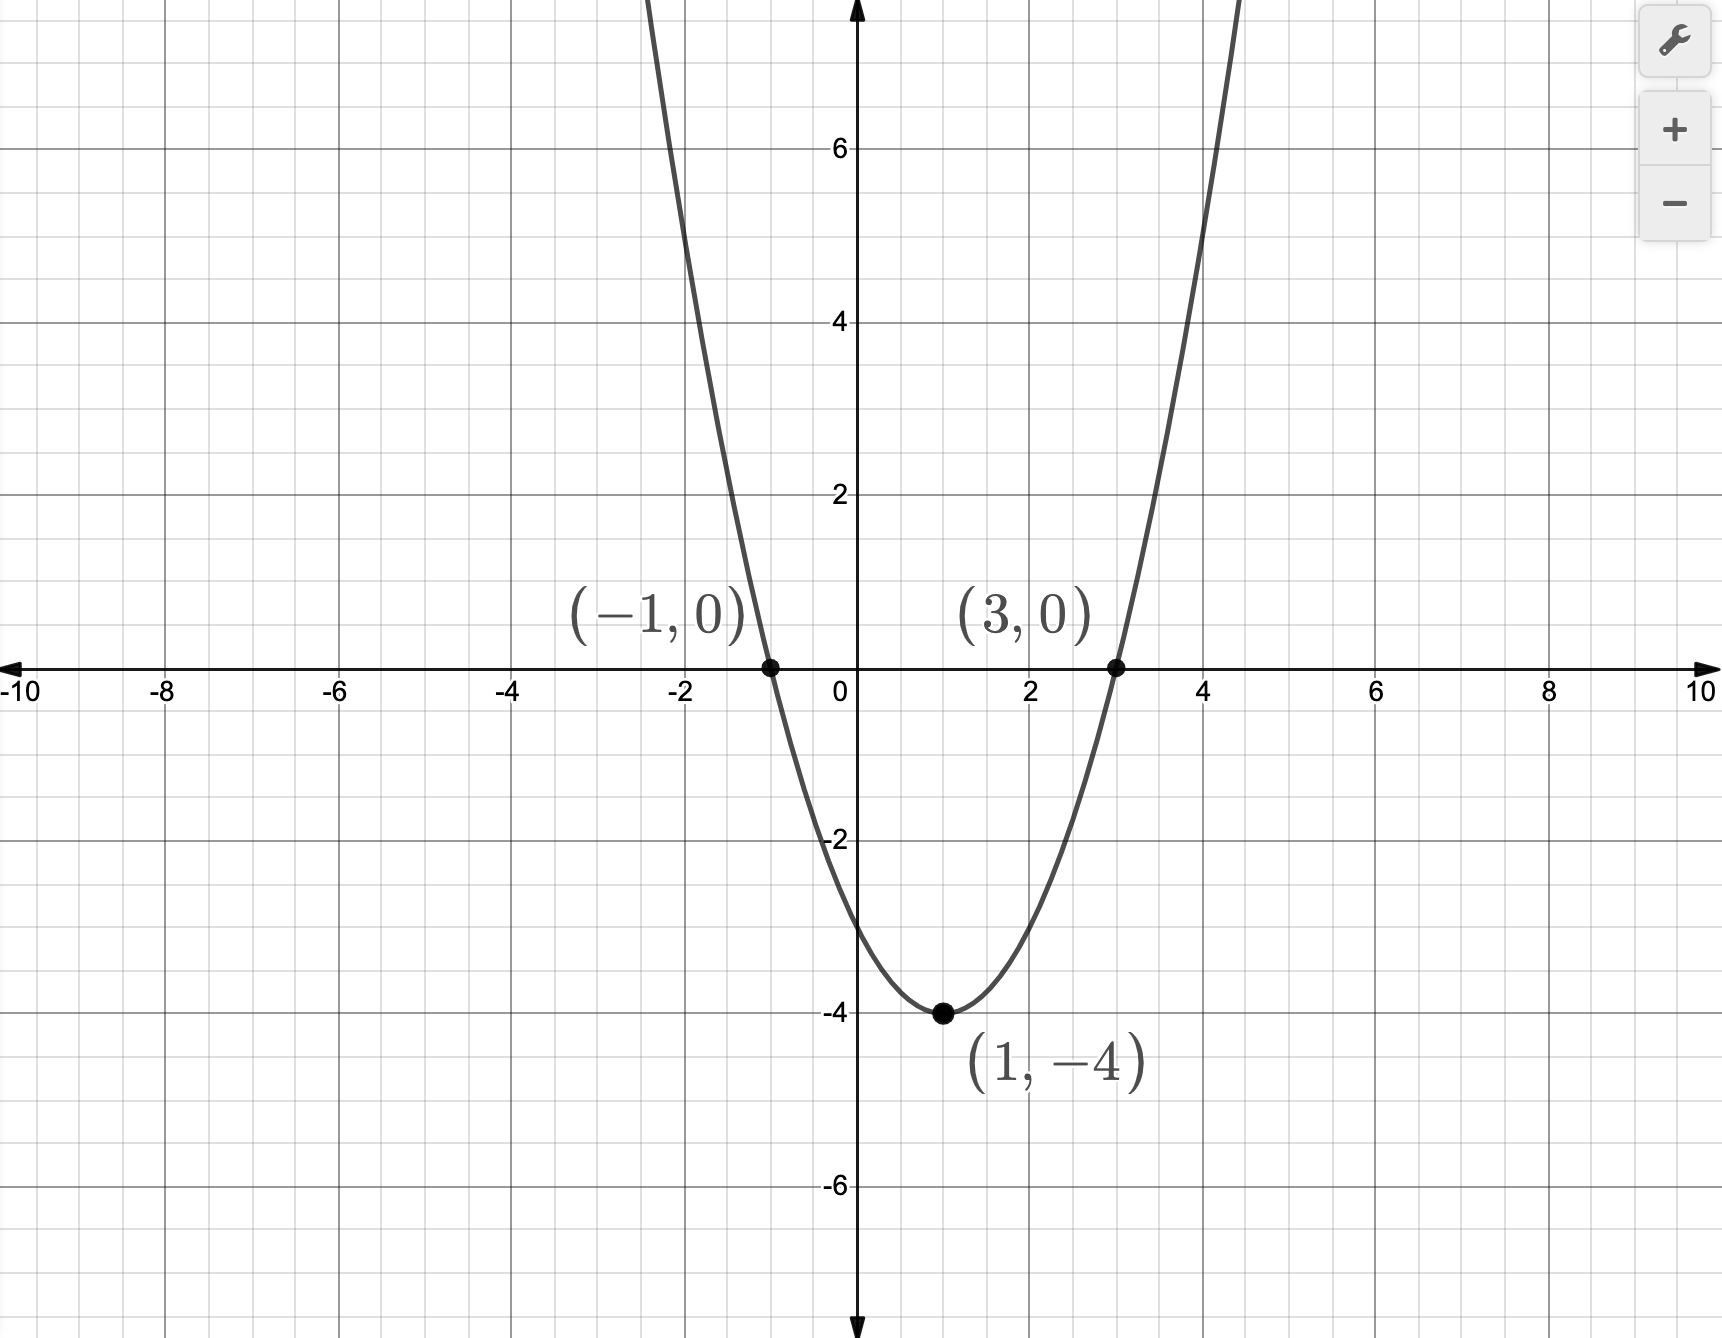
\includegraphics[scale=0.2]{4_1_025.png}
			\end{center}
		\end{figure}
	\end{enumerate}
\end{frame}

\begin{frame}
	\frametitle{Example (cont.)}
		\begin{enumerate}
			\item[]<1->find the zeros of $f(x)$:
			\item[]<2-> \textsc{Solution:} $x=-1, 3$;
			\item[]<3->the $x-$intercepts:
			\item[]<4->\textsc{Solution:} $x=-1, 3$;
			\item[]<5->the $y-$intercept:
			\item[]<6->\textsc{Solution:} $y=-3$;
			\item[]<7->the minimum:
			\item[]<8->\textsc{Solution:} $y=-4$;
			\item[]<9->the maximum:
			\item[]<10->\textsc{Solution:} $\infty$;
			\item[]<11->the domain:
			\item[]<12->\textsc{Solution:} $(-\infty, \infty)$;
			\item[]<13->the range:
			\item[]<14->\textsc{Solution:} $[-4, \infty)$.
		\end{enumerate}
\end{frame}

\begin{frame}
	\frametitle{Example}
	\begin{enumerate}
		\item[]<1-> Given
		\[
			g(x)=x^{3}+2x^{2}-11x-12=(x+4)(x+1)(x-3),
		\]
		\item[]<2->
		\begin{figure}
			\begin{center}
				\caption{$g(x)=x^{3}+2x^{2}-11x-12$}
				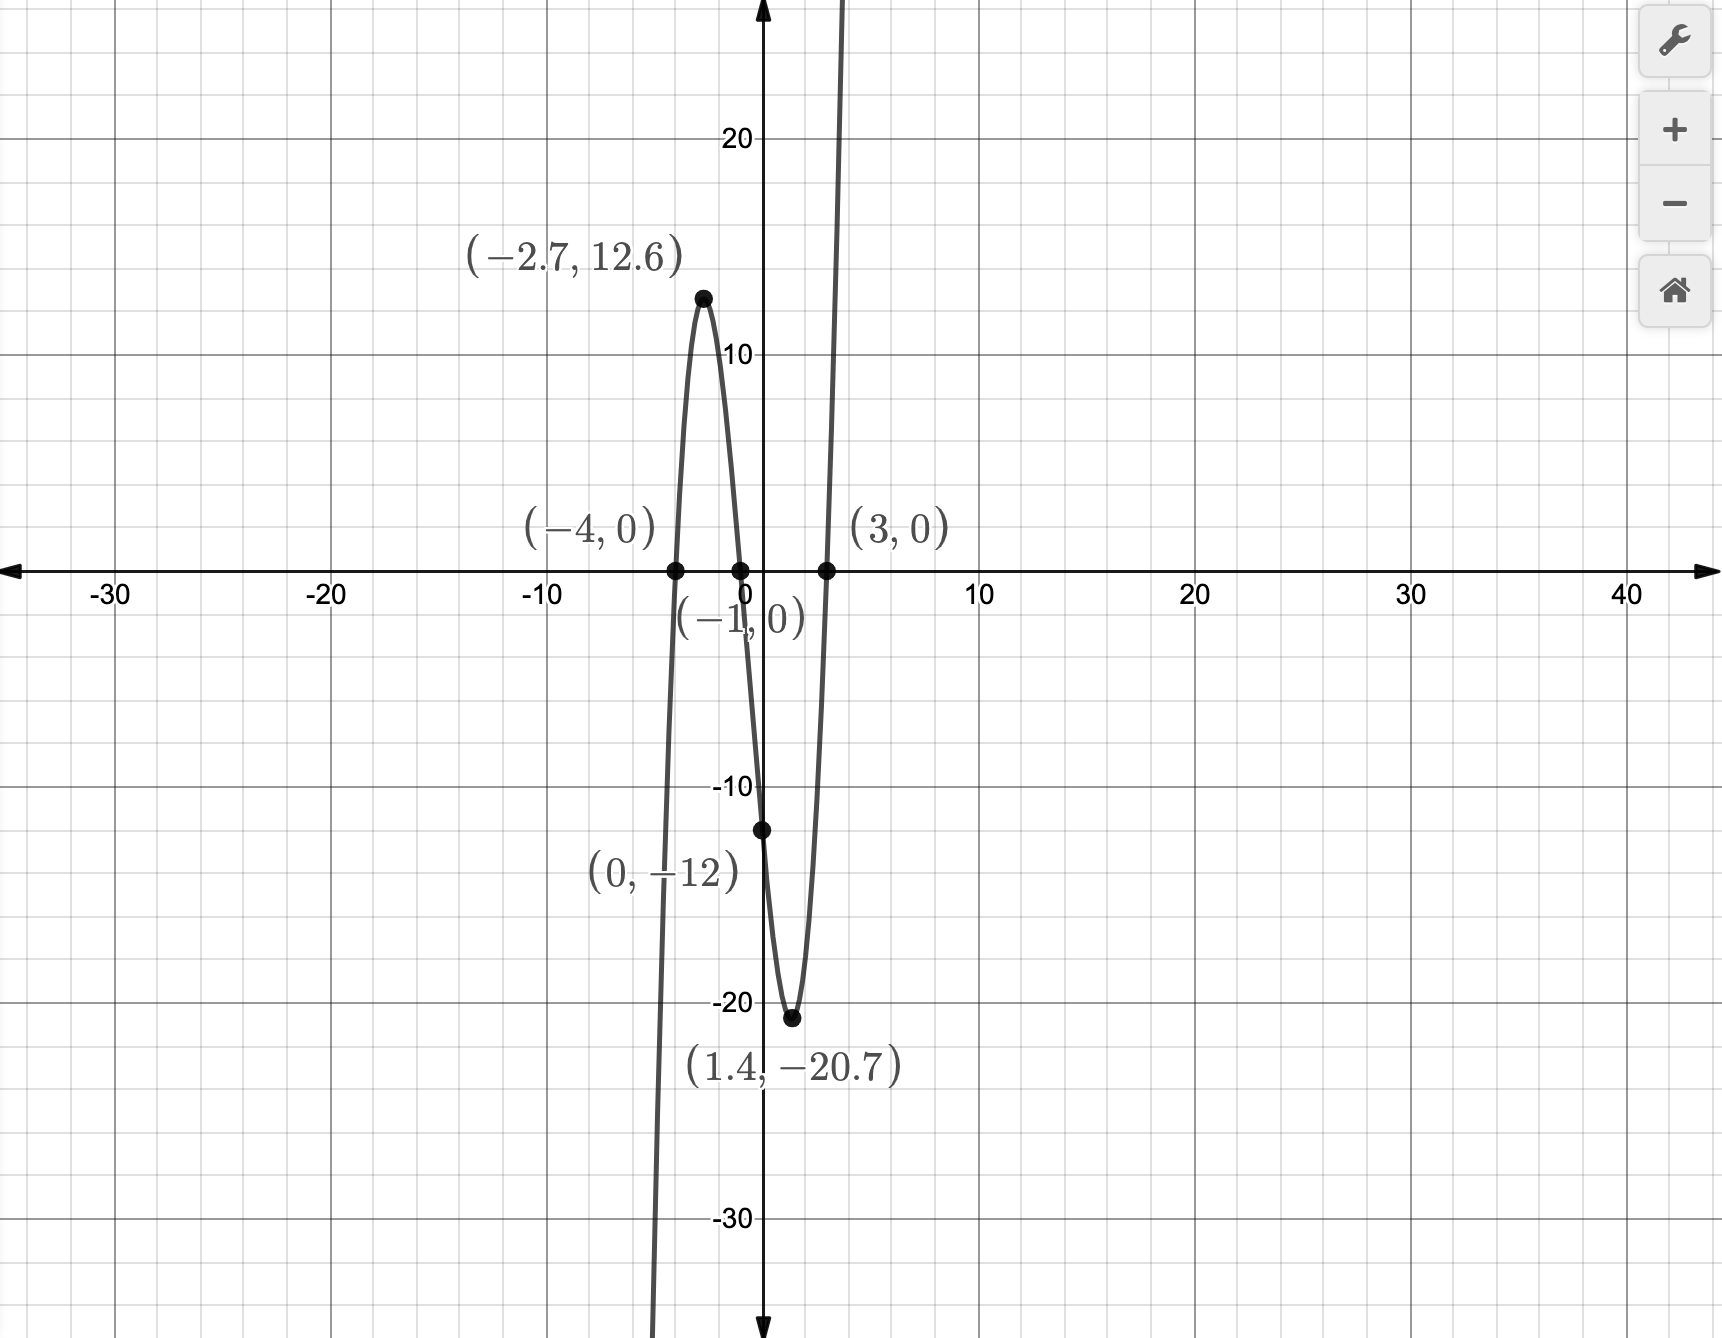
\includegraphics[scale=0.2]{4_1_050.png}
			\end{center}
		\end{figure}
	\end{enumerate}
\end{frame}

\begin{frame}
	\frametitle{Example (cont.)}
		\begin{enumerate}
			\item[]<1->find the zeros of $g(x)$:
			\item[]<2-> \textsc{Solution:} $x=-4, -1, 3$;
			\item[]<3->the $x-$intercepts:
			\item[]<4->\textsc{Solution:} $x=-4, -1, 3$;
			\item[]<5->the $y-$intercept:
			\item[]<6->\textsc{Solution:} $y=-12$;
			\item[]<7->the minimum:
			\item[]<8->\textsc{Solution:} $-\infty$;
			\item[]<9->the maximum:
			\item[]<10->\textsc{Solution:} $\infty$;
			\item[]<11->the domain:
			\item[]<12->\textsc{Solution:} $(-\infty, \infty)$;
			\item[]<13->the range:
			\item[]<14->\textsc{Solution:} $(-\infty, \infty)$.
		\end{enumerate}
\end{frame}

\begin{frame}
	\frametitle{Examples of Polynomial Functions}
	\begin{enumerate}
		\item[]<1->
		\begin{figure}
			\begin{center}
				\caption{Polynomial Functions}
				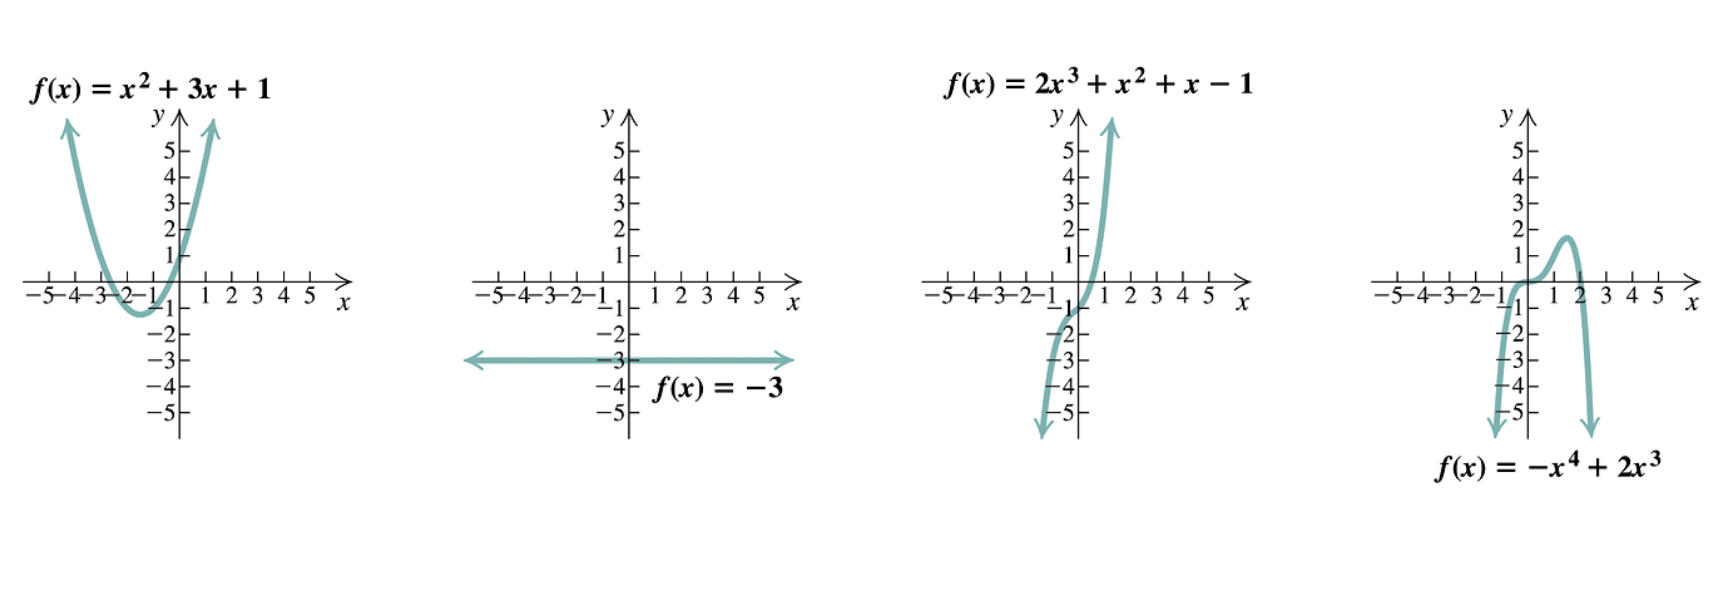
\includegraphics[scale=0.35]{4_1_1.png}
			\end{center}
		\end{figure}
	\end{enumerate}
\end{frame}

\begin{frame}
	\frametitle{Examples of Nonpolynomial Functions}
	\begin{enumerate}
		\item[]<1->
		\begin{figure}
			\begin{center}
				\caption{Nonpolynomial Functions}
				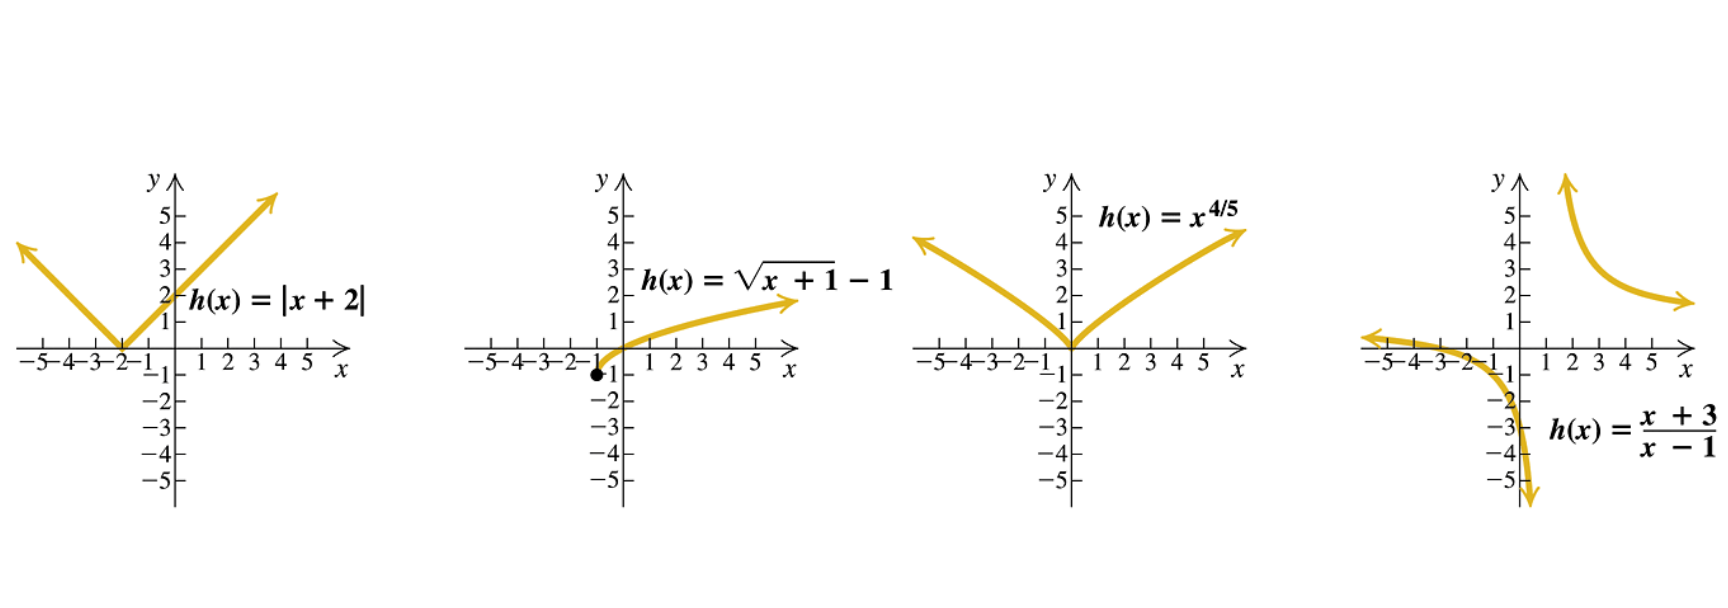
\includegraphics[scale=0.35]{4_1_2.png}
			\end{center}
		\end{figure}
	\end{enumerate}
\end{frame}


\end{document}
